\documentclass[aps,pra,twocolumn,reprint,amsmath,amssymb]{revtex4-2}

\usepackage{graphicx}
\usepackage{booktabs}
\usepackage{siunitx}
\usepackage[colorlinks=true,linkcolor=blue,citecolor=blue,urlcolor=blue]{hyperref}
\usepackage{float}
\usepackage{xcolor}

\begin{document}

\title{Free Dispersive Conditional-Phase Accumulation: A Minimal Model Validation Note}
\author{Execution Engineer}
\date{\today}

\begin{abstract}
We examine the smallest cQED question needed to validate the repository study loop at the model level: whether first-order dispersive idle evolution alone can generate a relative qubit phase of $\pi$ between the cavity $n=0$ and $n=1$ manifolds in finite time. Starting from the rotating-frame Hamiltonian $H/\hbar = \chi \hat{n} |e\rangle\langle e|$, the relative phase obeys $\Delta\phi_{1,0}(t) = -\chi t$, so the first positive crossing occurs at $t_{\pi} = \pi/|\chi|$. For the representative dispersive shift $\chi/2\pi = \SI{-2.84}{\mega\hertz}$, this gives $t_{\pi} = \SI{176.056338}{\nano\second}$. Two lightweight numerical checks implemented with the repository simulation framework reproduce the analytic trace over 51 sampled idle times: a closed-form idle-evolution helper and an independent static-Hamiltonian evolution in the rotating frame. The maximum wrapped mismatch between either numerical path and the analytic law is $8.882\times 10^{-16}\,\mathrm{rad}$, while raising the cavity cutoff from 2 to 3 Fock states changes the helper trace by $0\,\mathrm{rad}$. This note therefore validates the sign convention and basic free-evolution behavior of the model used in the study workflow. The scope is deliberately narrow: it is a closed-system first-order identity check, not a hardware-realism or gate-performance claim.
\end{abstract}

\maketitle

\section{Introduction}
Conditional phases generated by dispersive qubit-cavity coupling are a standard element of circuit QED reasoning~\cite{blais2004cavity,koch2007transmon}. For this repository, however, even a textbook identity is useful when it closes an end-to-end validation chain: analytic model, framework-backed computation, saved artifacts, reproducibility notebook, and report. The present study is intentionally scoped to that minimal target. Rather than claiming a new physical result, it asks whether the first-order dispersive model used throughout the repository produces the expected relative qubit phase between the $n=0$ and $n=1$ cavity manifolds under free idle evolution, and whether that behavior is reproduced by two independent numerical paths in the local simulation framework~\cite{cqedsim2025}.

The study is therefore a model-validation note, not a hardware-level benchmark. No microscopic coupling $g$ or detuning $\Delta$ is inferred here, and no statement is made about experimentally realized gate fidelity, decoherence, or beyond-dispersive corrections. The report first derives the phase law from the minimal Hamiltonian, then compares the analytic result with closed-form and Hamiltonian-evolution checks, and finally records the quantitative validation and reproducibility evidence.

\section{System and Methods}

\subsection{Hamiltonian and Analytic Preliminary}
The study starts from the first-order dispersive Hamiltonian in the frame rotating at the bare qubit and cavity frequencies,
\begin{equation}
\frac{H}{\hbar} = \chi \hat{n} |e\rangle\langle e|,
\label{eq:hamiltonian}
\end{equation}
where $\hat{n}$ is the cavity photon-number operator and $\chi$ is the qubit-storage dispersive shift. For cavity manifold $n$, the excited branch acquires phase
\begin{equation}
\phi_n(t) = -\chi n t.
\label{eq:branch_phase}
\end{equation}
The relative phase between the $n=1$ and $n=0$ manifolds is therefore
\begin{equation}
\Delta\phi_{1,0}(t) = \phi_1(t) - \phi_0(t) = -\chi t,
\label{eq:relative_phase}
\end{equation}
which reaches $\pi$ for the first positive time at
\begin{equation}
t_{\pi} = \frac{\pi}{|\chi|}.
\label{eq:tpi}
\end{equation}
Equations~\eqref{eq:relative_phase} and~\eqref{eq:tpi} are the central analytic claims tested below.

The controlled approximations are explicit. The calculation retains only the first-order dispersive term, neglects decoherence and drive-induced dynamics, and focuses on the low-occupation manifolds $n=0$ and $n=1$. Because the study begins from Eq.~\eqref{eq:hamiltonian} rather than from a microscopic Jaynes-Cummings model, it does not estimate a coupling-to-detuning ratio and does not claim to quantify the validity window of any specific hardware realization.

\subsection{Representative Parameters}
Table~\ref{tab:parameters} lists the representative parameters used for the numerical checks. The frequency values are chosen to remain consistent with the repository defaults, while the physical claim itself depends only on the dispersive shift in Eq.~\eqref{eq:tpi}.

\begin{table}[t]
\caption{Representative parameters used in the model-validation probe.}
\label{tab:parameters}
\begin{tabular}{lll}
\toprule
Parameter & Value & Unit \\
\midrule
Qubit frequency & 6.150 & GHz \\
Cavity frequency & 5.241 & GHz \\
Qubit anharmonicity & -255 & MHz \\
Dispersive shift $\chi/2\pi$ & -2.84 & MHz \\
Cavity self-Kerr $K/2\pi$ & -28 & kHz \\
Qubit Hilbert-space dimension & 2 & levels \\
Cavity cutoffs & 2, 3 & Fock states \\
Idle-time samples & 51 & dimensionless \\
\bottomrule
\end{tabular}
\end{table}

\subsection{Computational Approach}
Two numerical paths are used. The first evaluates a closed-form idle-evolution helper provided by the repository simulation framework. This path is essentially a sign-convention audit for Eq.~\eqref{eq:relative_phase}. The second constructs the static Hamiltonian in the same rotating frame and evaluates the idle evolution directly from the corresponding unitary. Because the two numerical routes share the same underlying model but not the same helper interface, their agreement removes the main methodological ambiguity present in a helper-only confirmation.

The calculation remains intentionally lightweight. The scan covers 51 evenly spaced times over $[0, 2 t_{\pi}]$, and both numerical paths use direct unitary evaluation rather than time-step integration. The full script runtime for the saved artifact set is \SI{1.076}{\second} on CPU.

\section{Results}
Figure~\ref{fig:phase_agreement} compares the analytic phase law with the two numerical evaluations. The upper panel shows that the closed-form helper and the static-Hamiltonian evolution are visually indistinguishable from Eq.~\eqref{eq:relative_phase} across the full scan. The lower panel plots the absolute wrapped residuals, which remain at the level of floating-point roundoff. For the representative shift in Table~\ref{tab:parameters}, Eq.~\eqref{eq:tpi} predicts a first positive crossing at \SI{176.056338}{\nano\second}, and the sampled numerical traces reproduce that value exactly to the printed precision.

\begin{figure}[t]
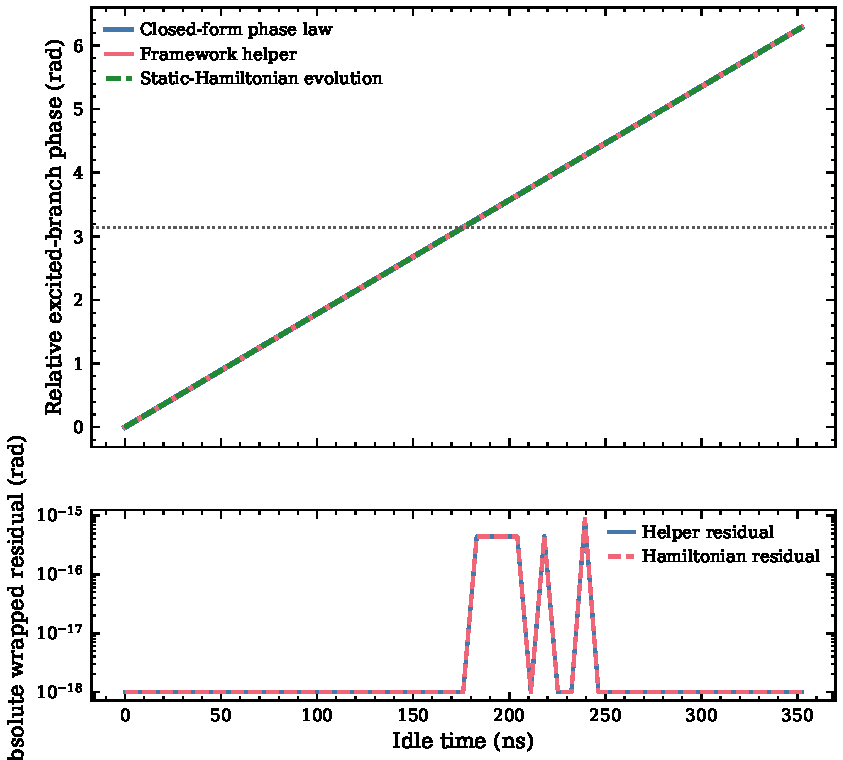
\includegraphics[width=\columnwidth]{../figures/phase_difference_hamiltonian_cross_check.pdf}
\caption{Comparison of the closed-form phase law, the framework helper, and the independent static-Hamiltonian evolution. Upper panel: relative excited-branch phase between the $n=1$ and $n=0$ manifolds during free idle evolution. Lower panel: absolute wrapped residuals relative to the analytic law. The first positive $\pi$ crossing occurs at \SI{176.056338}{\nano\second}.}
\label{fig:phase_agreement}
\end{figure}

The result is physically straightforward but operationally useful. Under the first-order dispersive Hamiltonian of Eq.~\eqref{eq:hamiltonian}, free idle evolution alone is sufficient to accumulate a conditional phase of $\pi$ whenever $\chi \neq 0$. Within the present scope, the numerical role is not to discover a new effect but to verify that the repository implementation reproduces the expected model behavior with machine-precision internal consistency.

\section{Validation}

\subsection{Sanity Checks}
The saved traces satisfy the expected zero-time condition $\Delta\phi_{1,0}(0)=0$ and follow the linear phase law of Eq.~\eqref{eq:relative_phase}. The closest sampled point to the first positive $\pi$ crossing occurs at \SI{176.056338028169}{\nano\second}, where the analytic, helper-based, and Hamiltonian-evolution phases all equal $3.14159265359\,\mathrm{rad}$ to the printed precision.

\subsection{Convergence}
The Hilbert-space convergence check is quantitative. Raising the cavity cutoff from 2 to 3 Fock states changes the wrapped helper trace by $0\,\mathrm{rad}$ over all 51 sampled times. Figure~\ref{fig:cutoff_scan} in Appendix~A overlays the two cutoff choices with the analytic law. No time-step convergence sweep is required because both numerical paths use direct unitary evaluation rather than an ordinary-differential-equation solver.

\subsection{Independent Evidence and Comparison Scope}
The maximum wrapped mismatch between the analytic law and the helper path is $8.882\times10^{-16}\,\mathrm{rad}$, and the same bound holds for the analytic law versus the static-Hamiltonian path. The helper and Hamiltonian traces differ by $0\,\mathrm{rad}$ after phase wrapping over the entire scan. These numbers satisfy the internal validation target for a deterministic model-level check.

An external literature comparison is not part of the present scope. This report does not attempt to benchmark a device or an optimization protocol against published data; it instead validates that the local first-order dispersive implementation reproduces its own analytic limit.

\section{Discussion}
The revised evidence chain supports a narrow but clean conclusion. The first-order dispersive identity of Eq.~\eqref{eq:tpi} is reproduced not only by a closed-form helper but also by direct static-Hamiltonian evolution in the rotating frame. That agreement shows that the phase accumulation reported here is not an artifact of one convenience interface. The additional Hamiltonian check also resolves the main methodological weakness identified in the previous review iteration.

The scope should nevertheless remain explicit. Because the study starts from Eq.~\eqref{eq:hamiltonian}, it does not test where the dispersive approximation breaks down, how decoherence modifies the idle phase, or how a pulse-level implementation would perform in a calibrated device. The contribution is therefore repository-facing: a compact validation note that the minimal model, saved artifacts, and reporting pipeline remain mutually consistent.

\section{Conclusion}
For the first-order dispersive Hamiltonian of Eq.~\eqref{eq:hamiltonian}, the relative qubit phase between the cavity $n=1$ and $n=0$ manifolds evolves as $\Delta\phi_{1,0}(t) = -\chi t$, so the first positive conditional-phase crossing occurs at $t_{\pi} = \pi/|\chi|$. With the representative shift $\chi/2\pi = \SI{-2.84}{\mega\hertz}$, the model gives \SI{176.056338}{\nano\second}. A closed-form framework helper and an independent static-Hamiltonian evolution both reproduce the analytic trace to a maximum wrapped mismatch of $8.882\times10^{-16}\,\mathrm{rad}$, while the minimal cavity-cutoff check changes the result by $0\,\mathrm{rad}$. The study therefore completes its intended role as a minimal model-validation note for the repository workflow.

\section{Limitations and Future Work}

\subsection{Known Limitations}
The study is restricted to a closed-system first-order dispersive Hamiltonian and therefore omits decoherence, higher-order dispersive corrections, and any hardware-transfer or pulse-shaping effects. It also does not derive a microscopic coupling-to-detuning ratio, so its claims stop at model-level consistency rather than dispersive-regime realism for a specific device.

\subsection{Suggested Improvements}
\begin{itemize}
\item \textbf{[P1 | MEDIUM]} Add a controlled beyond-first-order extension, such as a higher-order dispersive correction or weak self-Kerr deformation, to quantify when Eq.~\eqref{eq:tpi} ceases to be exact.
\item \textbf{[P2 | MEDIUM]} Introduce a dissipative idle-evolution model to measure how dephasing or cavity loss broadens the effective $\pi$ crossing.
\item \textbf{[P3 | LOW]} Promote the present deterministic checks to an automated regression target so future framework changes can be screened against the saved phase traces.
\end{itemize}

\subsection{Open Questions}
The main unresolved question is how quickly the ideal relation $t_{\pi}=\pi/|\chi|$ deforms once higher-order dispersive structure or decoherence is included while keeping the same representative parameter scale.

\bibliographystyle{apsrev4-2}
\bibliography{references}

\appendix

\section{Detailed Results and Data}
The saved scan covers 51 evenly spaced idle times over $[0, 2 t_{\pi}] = [0, \SI{352.112676}{\nano\second}]$. Table~\ref{tab:digest} records the compact quantitative digest used throughout the main text. Figure~\ref{fig:cutoff_scan} shows that the helper traces for cavity cutoffs 2 and 3 remain exactly overlapped after phase wrapping, consistent with the zero-difference convergence statement in the validation section.

\begin{table}[h]
\caption{Compact numerical digest for the saved probe outputs.}
\label{tab:digest}
\begin{tabular}{ll}
\toprule
Quantity & Value \\
\midrule
First positive $\pi$ crossing & \SI{176.056338}{\nano\second} \\
Maximum wrapped helper residual & $8.882\times10^{-16}\,\mathrm{rad}$ \\
Maximum wrapped Hamiltonian residual & $8.882\times10^{-16}\,\mathrm{rad}$ \\
Maximum wrapped cutoff difference & $0\,\mathrm{rad}$ \\
Saved runtime & \SI{1.076}{\second} \\
\bottomrule
\end{tabular}
\end{table}

\begin{figure}[h]
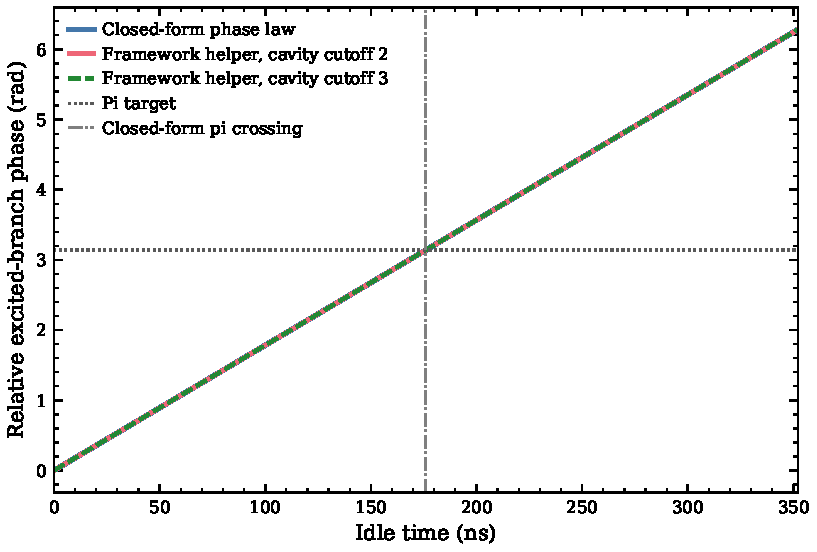
\includegraphics[width=\columnwidth]{../figures/phase_difference_vs_idle_time.pdf}
\caption{Cutoff-stability check for the helper-based evaluation. The traces for cavity cutoffs 2 and 3 overlap the analytic law over the entire scan, confirming that the low-occupation $n=0,1$ result is already converged at the minimal truncation used in the study.}
\label{fig:cutoff_scan}
\end{figure}

\section{Reproducibility}

\subsection{Representative Parameters}
The machine-readable summary stores the representative frequencies, anharmonicity, dispersive shift, self-Kerr, Hilbert-space dimensions, and scan range used to generate the saved outputs. The core value needed to reproduce the analytic result is the dispersive shift listed in Table~\ref{tab:parameters}.

\subsection{Modeling and Simulation Assumptions}
The calculation uses a two-level qubit, cavity cutoffs of 2 and 3 Fock states, closed-system evolution, and the rotating-frame first-order dispersive Hamiltonian of Eq.~\eqref{eq:hamiltonian}. The comparison observable is the wrapped relative phase modulo $2\pi$. No pulse sequence, optimizer, or stochastic sampling is involved.

\subsection{Reproduction Procedure}
\begin{enumerate}
	\item From the study root, run the self-contained study script listed in Table~\ref{tab:artifacts}.
	\item Confirm that the run updates the CSV data files, JSON artifacts, and dual-format figures in the study folders.
	\item Verify that the reported first positive $\pi$ crossing remains near \SI{176.056338}{\nano\second} and that the helper and Hamiltonian residuals stay at the level of floating-point roundoff.
	\item Open the reproducibility notebook listed in Table~\ref{tab:artifacts} for the load-first walkthrough and optional rerun path.
\end{enumerate}

\subsection{Saved Artifacts}
\begin{table*}[t]
\scriptsize
\caption{Machine-readable outputs and supporting files for the probe study.}
\label{tab:artifacts}
\begin{tabular*}{\textwidth}{@{\extracolsep{\fill}}llll}
\toprule
Filename & Format & Contents & Load example \\
\midrule
\shortstack[l]{\path{artifacts/}\\\path{free_dispersive_pi_probe_summary.json}} & JSON & \shortstack[l]{Representative parameters,\\analytic $t_{\pi}$, helper residuals,\\and cutoff-stability metrics} & \shortstack[l]{\path{json.loads(}\\\path{path.read_text())}} \\
\shortstack[l]{\path{artifacts/}\\\path{free_dispersive_hamiltonian_cross_check.json}} & JSON & \shortstack[l]{Static-Hamiltonian comparison\\metadata, extracted manifold shift,\\and residual summary} & \shortstack[l]{\path{json.loads(}\\\path{path.read_text())}} \\
\shortstack[l]{\path{data/}\\\path{phase_difference_samples.csv}} & CSV & \shortstack[l]{Sampled analytic and\\helper-based phase traces} & \shortstack[l]{\path{np.genfromtxt(}\\\path{path, names=True)}} \\
\shortstack[l]{\path{data/}\\\path{phase_difference_hamiltonian_cross_check.csv}} & CSV & \shortstack[l]{Sampled analytic, helper-based,\\and Hamiltonian traces plus residuals} & \shortstack[l]{\path{np.genfromtxt(}\\\path{path, names=True)}} \\
\shortstack[l]{\path{figures/}\\\path{phase_difference_vs_idle_time.pdf}} & PDF & \shortstack[l]{Vector cutoff-stability\\figure used in Appendix~A} & Open directly in a PDF viewer \\
\shortstack[l]{\path{figures/}\\\path{phase_difference_hamiltonian_cross_check.pdf}} & PDF & \shortstack[l]{Vector agreement-and-residual\\figure used in the main text} & Open directly in a PDF viewer \\
\shortstack[l]{\path{scripts/}\\\path{free_dispersive_pi_probe.py}} & Python & \shortstack[l]{Self-contained rerun script\\for the saved outputs} & \shortstack[l]{\path{python scripts/}\\\path{free_dispersive_pi_probe.py}} \\
\shortstack[l]{\path{scripts/}\\\path{reproducibility_notebook.ipynb}} & Notebook & \shortstack[l]{Load-first interactive\\walkthrough of the study outputs} & Open in VS Code or Jupyter \\
\bottomrule
\end{tabular*}
\end{table*}

\end{document}